\section{VNF Platform Architecture} \label{ARCH}

In this section, we introduce an architecture for VNF platforms which supports SFC chaining using NSH. The proposed architecture is designed to be flexible and technology agnostic. Ultimately, we expect this architecture to serve as a template for designing new systems and re-engineering existing ones.

\subsection{Architecture Overview}

Currently, there is no \textit{de facto} standard for the design and development of VNF platforms, from neither industry nor academia. VNF platforms, however, must be developed to meet multiple strict requirements (\textit{e.g.}, portability, performance, integration, management, and scalability), in order to fulfill the needs of modern networks. Furthermore, the NFV area is evolving, with new technologies being created continuously. Therefore, it is essential to design flexible solutions that support new NFV Enablers (\textit{i.e.}, existing frameworks and technologies that contribute to the development and implementation of NFV) from an ever increasing number of players in the NFV market.

VNF platforms must also be created with integration in mind. There are several systems (OSS/BSS, Hypervisors) and elements (NFVI, VNFM, EMS) that must work together with multiple VNFs in order to adequately provide virtualized network services \cite{GS-2014}.
%Furthermore, each running VNF can also be decomposed into multiple VNF Components (VNFCs), each performing some specific operation but acting in consonance with others to process network traffic.

%In this context, we propose a generic and flexible architecture for VNF platforms, (Figure~\ref{vnfGeneric}). The proposed platform consists of six main modules deployed on a host operating system (called here VNF Core): \textit{(i)} Virtual Network Subsystem, \textit{(ii)} Internal Router, \textit{(iii)} NSH Processor, \textit{(iv)} Packet Processing Subsystem, \textit{(v)} Management Agent, and \textit{(vi)} Extended  Agents. Each module performs specific operations within the VNF and can process network packets from both the data and control planes (depicted by solid lines) and the management plane (depicted by dashed lines). External interfaces to the VNF Core are also defined in the architecture to enable the use of virtualized resources (available in the NFVI) and to support both management and orchestration operations (by using EMS and VNFM systems).

%\subsection{Internal Modules}

%Each module of the architecture is designed to be loosely coupled and with well-defined access interfaces. In this way, each module can be redesigned or replaced as new software becomes available. Modules are described below:

%\begin{itemize}

%\item \textbf{Virtual Network Subsystem} (VNS) -- This module is responsible for accessing the Virtual Network Interface Controllers (VNICs) -- provided by the hypervisor -- for sending/receiving network packets. Typically, this operation, when executed by the native network stack in traditional operating systems, is not optimized to support the performance requirements of high-speed networks (\textit{e.g.}, 40GbE/100GbE). To tackle this problem, several packet acceleration tools (\textit{e.g.}, Intel DPDK \cite{Intel-2014}, NetMap \cite{Rizzo-2012}, PacketShader \cite{Han-2010}, PF\_RING/DNA \cite{Ntop-2013}, and OpenOnload \cite{Solarflare-2013}) have been proposed and extensively evaluated. These systems can replace the traditional L2 Socket approach for traffic steering and present themselves as adequate solutions for NFV-based networks.

%\begin{figure}[!ht]
%    \centering
%    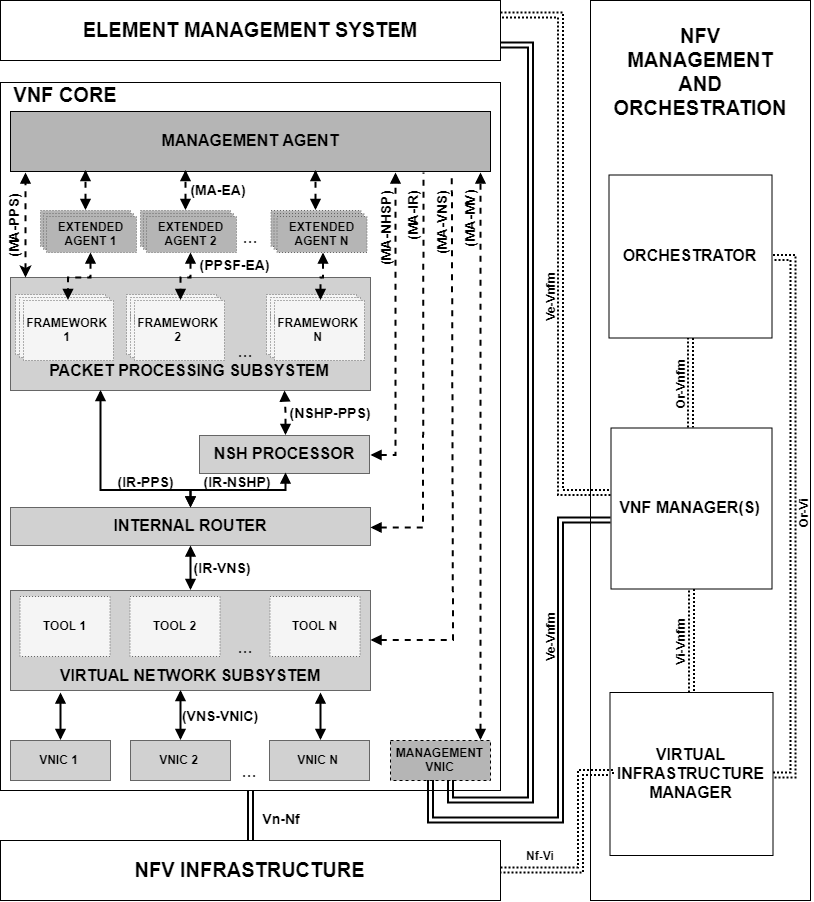
\includegraphics[width=0.48\textwidth]{images/FullArchitecture.png}
%    \caption{\label{vnfGeneric} VNF Platform Architecture}
%\end{figure}

%    \item \textbf{Internal Router} (IR) -- Once the network packets are captured by the VNS, they are forwarded internally to the VNF Core by the Internal Router. The configuration of this module is the responsibility of the Management Agent (discussed later), which specifies the order of processing among the several VNFCs. Once the Internal Router is initialized, it uses communication channels (\textit{e.g.}, using shared memory, pipes, sockets) to forward the network packets between the VNS, the Packet Processing Subsystem (PPS), and the NSH Processor (NSHP). The use of an IR allows VNFCs to be created individually.

%    \item \textbf{NSH Processor} (NSHP) -- the IETF specified the Network Service Header (NSH) that is inserted in packets/frames to provide service function paths \cite{Quinn-2018}. However, despite its advantages, the use of NSH is optional to steer traffic across multiple VNFs. In order to support both cases, we define the NSH Processor, which provides an abstraction for the network functions regarding the existence of NSH packets. Specifically, when the Internal Router detects a NSH packet, it forwards the packet to be processed by the NSHP. Alternatively, the network packet is forwarded directly to the corresponding VNFC. NSHP acts on the specific NSH fields that may be modified when traversing a network path (\textit{i.e.,} the Service Index - SI; and Context Header - CH). NSHP provides the following operations: NSH removal, NSH reinsertion, CH retrieval, and CH update.

%    \item \textbf{Packet Processing Subsystem} (PPS) -- This module corresponds to the development frameworks used to implement network functions. Basically, these frameworks include applications (\textit{e.g.}, Click Modular Router \cite{Kohler-2000} and Vector Packet Processing \cite{Cisco-2018}), programming languages (\textit{e.g.}, C, C++, Python), libraries (\textit{e.g.}, Scapy, libtins, libnet), or even single routines that support the construction and handling of network packets.

%    \item \textbf{Management Agent} (MA) -- The primary goal of a MA is to monitor and control the execution of VNFs. Furthermore, it is also responsible for coordinating the execution of all internal modules of the VNF platform. MA provides five main operations: request, retrieve, start, stop, and monitor. The request operation receives a VNF Package (VNFP) \cite{IFA-2018} from the network operator and deploys the specified VNF instance. Once a VNF is executing, retrieve operations can be used to gather information about the VNF instance (\textit{e.g.}, VNF ID, network interfaces). The start and stop operations are responsible for the VNF lifecycle management. Finally, the monitoring operation is responsible for measuring performance indicators from the VNF Core (\textit{e.g.}, CPU, memory, and network usage) and providing information retrieved from the extended agents deployed in the VNF platform.

%    \item \textbf{Extended Agent} (EA) -- The module is controlled by the Management Agent and is used to monitor/control each network function or component. It is supposed to be developed by the creator of the VNF/VNFC, as it acts on the individual management data of those implementations (\textit{e.g.}, number of discarded packets by a firewall). This module must provide at least one standard operation which we call ``list''. This operation is used by MA to discover all the management data that can be accessed by network operators.

%\end{itemize}

 All the described modules are controlled by the MA, which upon receiving a VNFP (MA-MV interface), does the validation, extracts the relevant information for deploying the VNF, and configures the internal modules accordingly. For example, VNFP may contain information regarding the set of VNFCs that compose a VNF, which is essential for the Internal Router to forward the traffic to the proper components. The initial request for VNF deployment must also provide more specific information, such as the extended agents to be instantiated together with the network functions.

The Management Agent is also responsible for extracting the implementation source code of the VNFCs from the VNFP, request the Packet Processing Subsystem to create the associated communication channels, and to start the execution of VNFCs (Figure \ref{vnfGeneric} MA-EA and PPSF-EA). Once this operation concludes, PPS returns a success/failure confirmation to the Management Agent (MA-PPS). In case of failures, rollback mechanisms may be employed to abort the instantiation process properly. When NSH is used, the Management Agent starts the NSH Processor (MA-NSHP). NSHP then creates a communication channel with the Packet Processing Subsystem (NSHP-PPS) to allow the network functions to access the NSH context header. VNICs are connected to the Virtual Network Subsystem (VNS-VNIC) based on the original request specified in the VNFP, processed by the MA (MA-VNS). The overall configuration of the VNF Platform is depicted in Figure \ref{FIG:CONF}.

%\begin{figure} [!h]
%\centering
%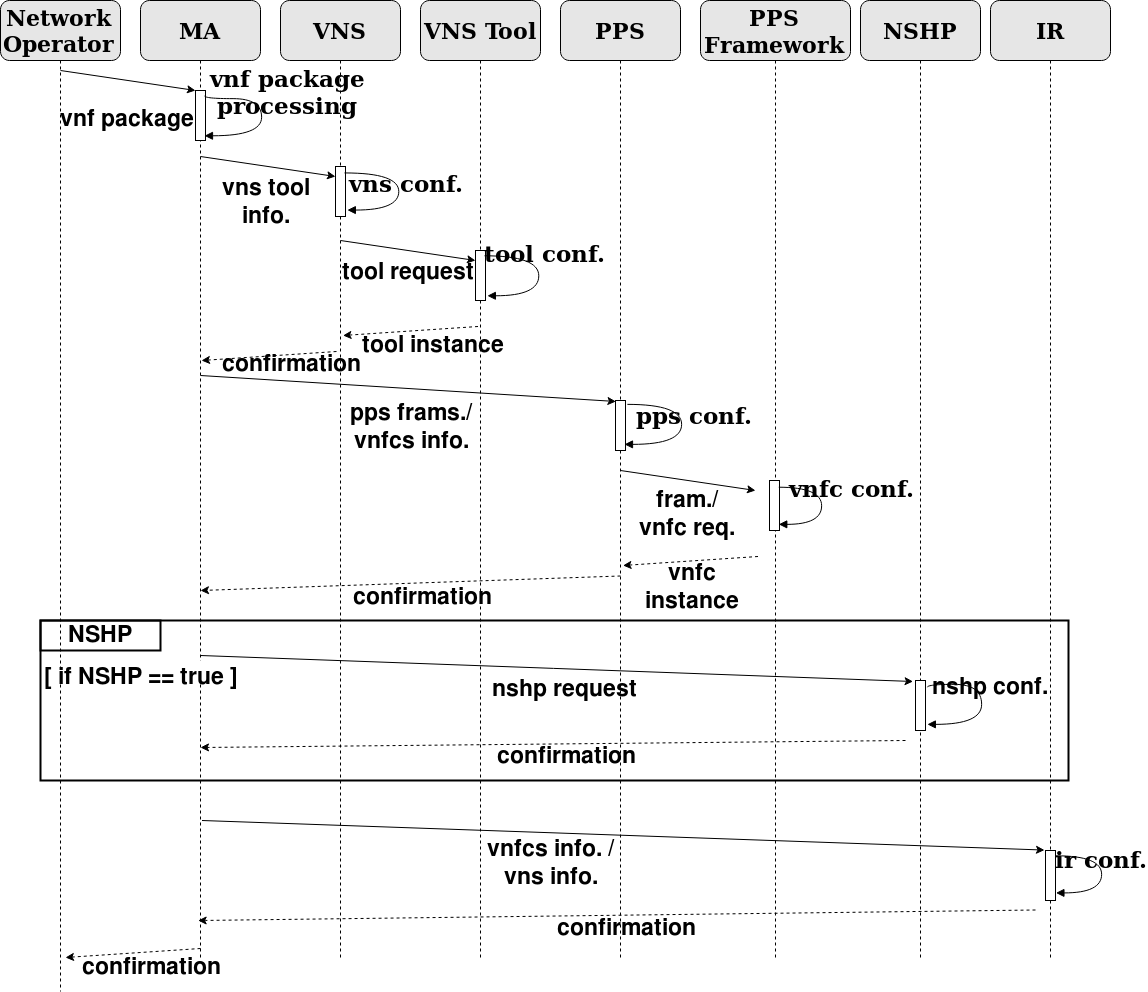
\includegraphics[width=\linewidth]{images/Configuration.png}
%\caption{Configuration Process}
%\label{FIG:CONF}
%\end{figure}

Finally, the Internal Router is initiated with two default communication channels: IR-VNS and IR-PPS. The former is used by the IR to retrieve network packets from the VNS, while the latter is used by VNFCs to access the packets to be processed. A third connection labeled IR-NSHP is used (i) to remove the NSH before any VNFC and (ii) to reinsert the NSH after the last VNFC of the path.

The reference architecture described in this section defines the key modules responsible for the deployment of both VNFCs and SFCs \cite{Joel-2015}. We believe the architecture can provide a valuable reference for the design and development of VNF platforms, working as a guideline to integrate distinct modules in order to create complete solutions.
